%TEX root = ../dissertation.tex

\section{Wi-Fi Direct in Android}
\label{sec:wfd}

In this section, the current Wi-Fi Direct Android implementation will be described and analysed. There are small differences depending on the operating systems in which Wi-Fi Direct is being implemented, thus it is not possible to universally describe Wi-Fi Direct with more detail than the one used in Subsection \ref{subsection:wfd}.

In the next subsections, the details intrinsic to the Android operating system will be introduced and explained, followed by an in-depth description of various works on how to improve and expand the functionalities of this implementation.

\subsection{Wi-Fi Direct Star Formation}
\label{subsection:wfdstar}

As previously mentioned in Subsection \ref{subsection:wfd}, an ad hoc network is implemented in Wi-Fi Direct, by using a protocol for discovery and connection of the \gls{GO} with the \glspl{GM}. The \gls{GO} functions as a typical Wi-Fi \gls{AP}, managing the different communications of the \glspl{GM}.

\glspl{GO} are not predefined. It is during the group creation that the actual \gls{GO} is chosen, according to the specified parameters of the protocol, \textit{e.g.} battery percentage. This feature is relevant to manage the vitality of the network as a mesh of groups, since the \glspl{GO} can be chosen dynamically extending the life of the network.

After the process of the group creation, the \gls{GO} periodically sends a beacon to advertise the group, enabling other devices to discover and join the group. This advertisement is made in two different ways, either via Wi-Fi Direct, or via typical Wi-Fi. In the first way, devices discover the network via the Wi-Fi Direct discovery protocol, and join using the described set of actions. In the second way, the \gls{GO} announces the \gls{SSID} of the network and other devices, also known as legacy clients, connect via infrastructure mode Wi-Fi, using the \gls{SSID} and password, if set, to identify the \gls{GO}'s network. This leaves us with two different types of clients: legacy and normal. This differentiation will be the key to overcome the lack of multi-group interaction.

In Android devices, \gls{IP} addresses are predefined according to the function the device performs within the network. The \glspl{GO} are automatically assigned the following \gls{IP} address: 192.168.49.1/24, using \gls{DHCP}. Whenever a P2P or legacy client connects to the group, \gls{DHCP} is run again and the clients take an \gls{IP} address ranging from 192.168.49.2/24 to 192.168.49.254/24, chosen randomly to minimize the chance of conflicts. The \glspl{GO} are always assigned the same \gls{IP} addresses, unless they participate in another group as a \gls{GM} taking the same \gls{IP} as a regular client - see \cite{routeMultiGroup} for a more detailed explanation on this topic.

This technology is still not implemented to the best of its capacity in Android devices. The lack of a routing protocol that can establish multi-group communication, establishing a meshed network is an essential tool to achieve ad hoc networks. The current state of this technology in Android devices is a single group network with one-to-many links established from the \gls{GO} to the \glspl{GM}, which limits both the range and scalability of the network. Wi-Fi Alliance states that it is possible to overcome these limitations using stock devices, by creating software to allow for multi-group formation, although it is not standardized in Android's current version 7.0 "Nougat".

In the next section, a collection of developed work will be presented where the different authors propose different methodologies to overcome the lack of this feature in Android devices.

\subsection{Ad Hoc Networking}
\label{subsection:adhocnet}

C. Casetti \textit{et al.} propose in \cite{routeMultiGroup} a process to successfully form a meshed network, by allowing multiple groups to communicate. This proposition is based on stock Android, not requiring any "root" to be made to the devices, meaning all the actions will be performed in application layer, not envolving any changes in \gls{IP} addresses or \gls{MAC} interfaces.

The authors state that multi-group formation can be implemented by taking advantage of both virtual network interfaces of a device, \textit{i.e.}, the Wi-Fi or legacy interface and the Wi-Fi P2P interface, using each one to act as bridge in each group.

This said, upon experimentation, the following scenarios are not feasible in stock Android, due to the inability of creating a custom virtual network:

\begin{itemize}
\item a device is the \gls{GO} of one group and \gls{GM} in another,
\item a devices is the \gls{GO} of two or more groups,
\item a devices is a \gls{GM} in two or more groups (non-legacy).
\end{itemize}

Due to these limitations, the authors propose that a \gls{GO} be a legacy client in a different group, seen in Figure \ref{fig:mgrouprouting}:

\begin{figure}[ht]
	\noindent\makebox[\textwidth]
    {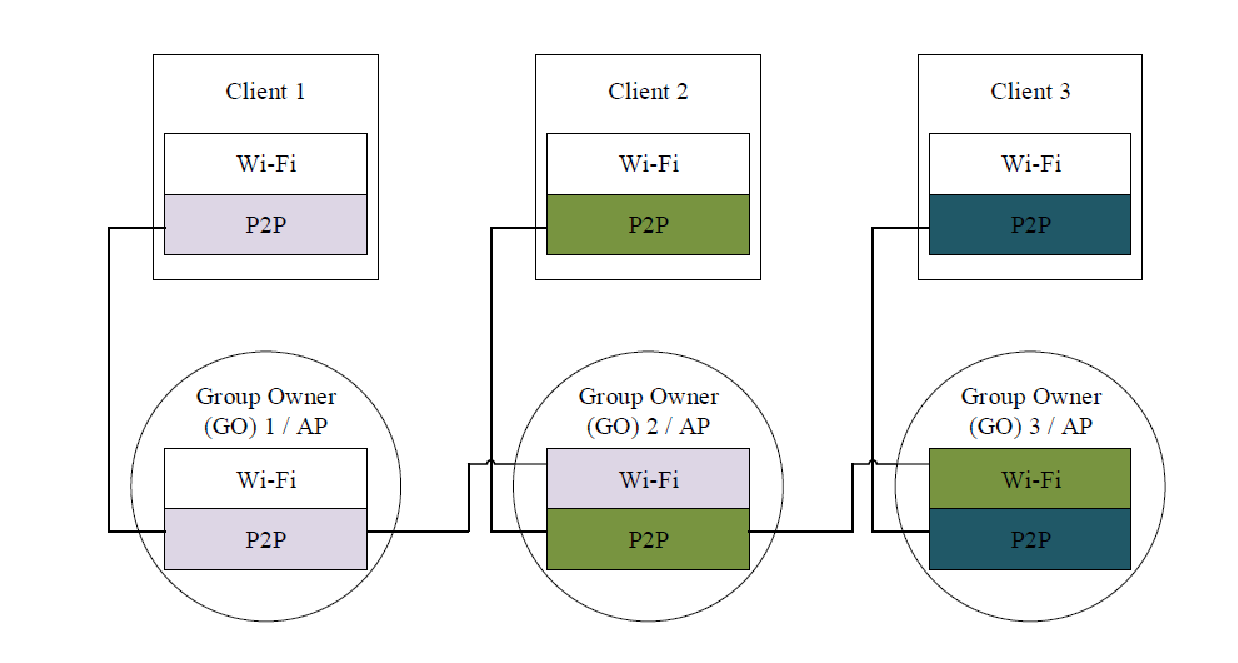
\includegraphics[width=1\textwidth]{images/mgrouprouting.pdf}}
	\caption{\label{fig:mgrouprouting} Multi-group physical topology with six devices (source: \cite{routeMultiGroup})}
\end{figure}

So, for each \gls{GO} two network interfaces are enabled, one is the conventional Wi-Fi and the other used for Wi-Fi Direct connection. The \gls{IP} addresses are assigned according to the previous description.

Two cases are distinguished by the authors: the \gls{GO} is not connected to any other group as a legacy client, which is the default topology of the network. In this case all connections are feasible, as Wi-Fi Direct has been implemented in order to provide full connectivity among all devices of a single group.

In the second case, the \gls{GO} is connected to another group as a legacy client as depicted in Figure \ref{fig:mgrouprouting} Groups 2 and 3, limiting data transfer to only a subset of D2D data. These limitation are due to two reasons, first the \gls{IP} conflict of both \glspl{GO}, who share the same address, 192.168.49.1, making the communication between two adjacent \glspl{GO} impossible. Secondly, when a \gls{GO} wants to send a unicast packet to any client, the packet is sent through the \gls{GO}'s Wi-Fi interface, due to Android's implementation of routing table entries in the \gls{GO}.

So in this case, client-to-\gls{GO} communication is allowed since client routing tables list only one interface and there are no conflicts, in \gls{GO}-to-client direction, bidirectional unicast communication is not allowed. Broadcast communication on the other hand is possible, since it is always sent through the \gls{GO}'s P2P interface. Although when they reach the \gls{GO} acting as a legacy client they are dropped due to the \gls{IP} address conflict mentioned above. Finally, client-to-client communication is bidirectional and sent through the client's P2P interface.

It is known from the first case that full connectivity among devices in a single group is allowed, even if one of the \glspl{GM} is a legacy client and \gls{GO} of another group. Based on this, the authors introduce the term relay node, which is used to describe this legacy client. The relay node is used to connect two groups. This node is chosen at random, upon the sending of a message from the \gls{GO} to one of its clients  chosen at random among those who do not act as \gls{GO} in another group. It is important to note that the authors state that this message must be broadcasted to avoid sending it through the Wi-Fi interface, the problem described above in the second case. These clients provide the communication backbone and provide connectivity to all other clients in the group, except from the ones acting as \glspl{GO} in another group.

\begin{figure}[ht]
	\noindent\makebox[\textwidth]
    {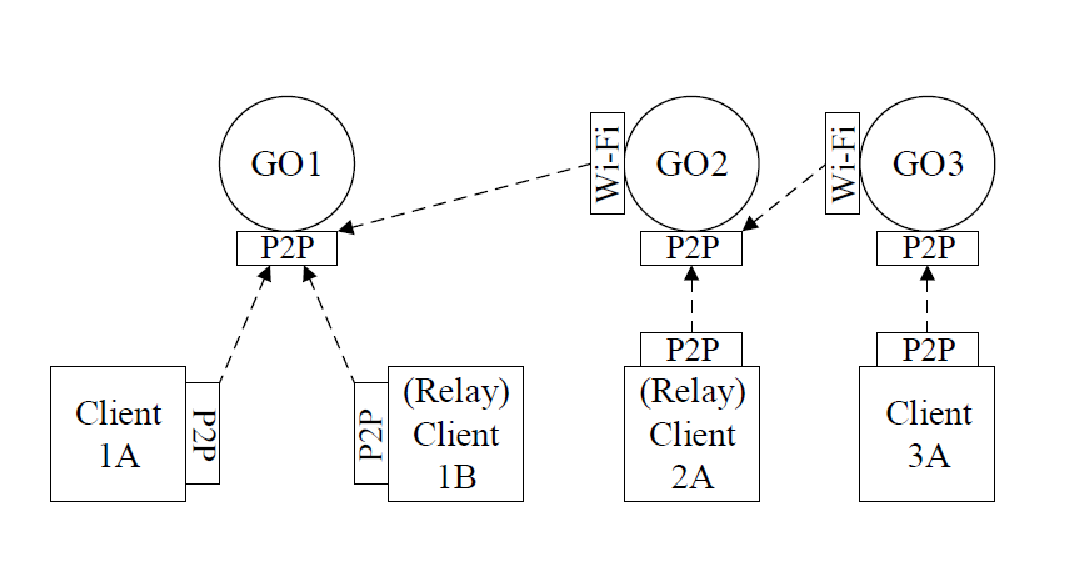
\includegraphics[width=0.9\textwidth]{images/1o1routingMGroup.pdf}}
	\caption{\label{fig:1o1routing} Example network topology with 3 Wi-Fi Direct groups. (source: \cite{routeMultiGroup})}
\end{figure}

Take Figure \ref{fig:1o1routing}, where only Wi-Fi Direct connections are represented, for instance. The procedure for Client 1A to send a packet to Client 3A is as follows: Client 1A encapsulates the data in the payload of a unicast \gls{UDP} packet and sends it to the relay Client 1B. The packet will be forwarded by GO1 to Client 1B, at the \gls{MAC} layer.

The packet is processed at the application layer and the payload is duplicated into a new \gls{UDP} packet. Sent directly to GO2's standard Wi-Fi interface \gls{IP} address. At the \gls{MAC} layer, the packet is sent to GO1, which sends the packet to GO2, via Wi-Fi direct.

The same process is repeated by GO2, but the packet is sent as a broadcast \gls{IP} packet through GO2's Wi-Fi Direct interface, to relay Client 2A. This client replicates the process of relay Client 1B, sending it to the \gls{IP} address of GO3's Wi-Fi interface.

Finally, GO3 processes the received packet and sends it to its destination with the correct payload, broadcasting it, similarly to the procedure of GO2.

This mechanism is used following the second case, where the \gls{GO} is connected to another group as a legacy client. With this mechanism the packet is successfully sent from group to group until its destination is reached, using a mix of unicast and broadcast communication.\newline

C. Funai \textit{et al.} propose a similar approach in \cite{multiHopD2D}. Their approach is to test two distinct possibilities for multi-group formation, as seen in Figures \ref{fig:mhopd2dgm} and \ref{fig:mhopd2dgo}, where "LC" stands for legacy client and refers to clients that use the classic Wi-Fi interface, instead of the P2P interface to connect to a group.

\begin{figure}[ht]
	\noindent\makebox[\textwidth]
    {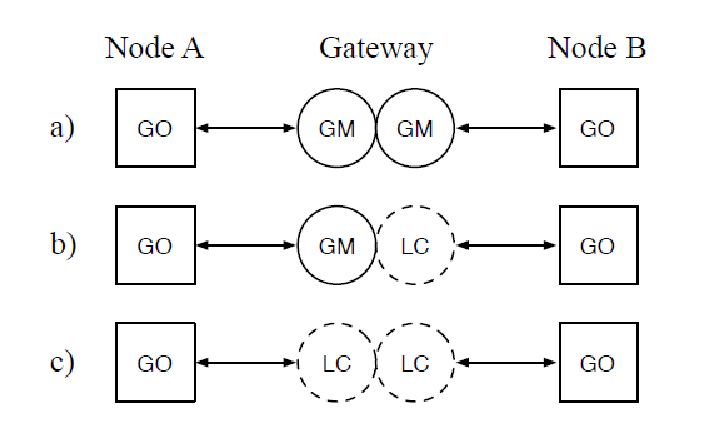
\includegraphics[width=0.6\textwidth]{images/mhop2d2GM.pdf}}
	\caption{\label{fig:mhopd2dgm} Multi-group communication scenarios where the gateway node acts as a client in two groups (source: \cite{multiHopD2D})}
\end{figure}
\begin{figure}[ht]
	\noindent\makebox[\textwidth]
    {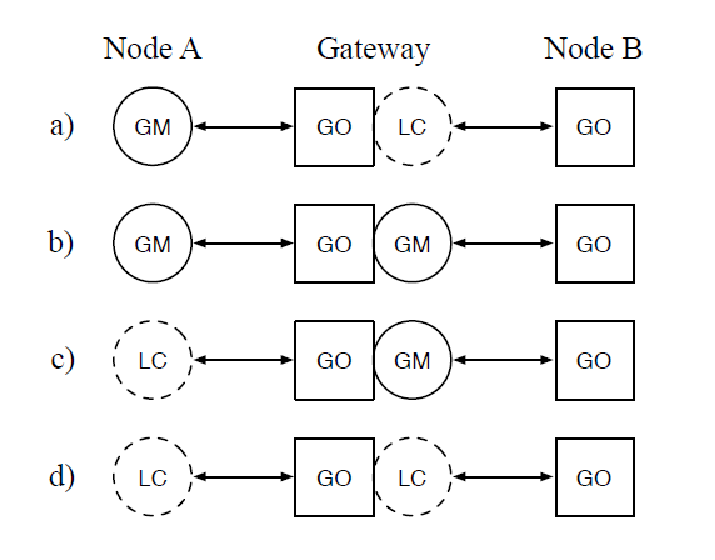
\includegraphics[width=0.6\textwidth]{images/mhop2d2GO.pdf}}
	\caption{\label{fig:mhopd2dgo} Multi-group communication scenarios where the gateway node acts as the GO in one group and as a client in the other (source: \cite{multiHopD2D})}
\end{figure}

The term gateway node is introduced, referring to the device that connects multiple groups. First by iteratively switching between the different P2P groups, relaying data between them. Secondly by using \gls{UDP}-based broadcast and a \gls{UDP}/\gls{TCP} hybrid solution to achieve multi-group communication. And finally by modifying the source code of the Android operating system.

The authors describe the limitations of stock Android, one of which the multi-group communication must be handled at the application layer and not at the network layer. Actions such as setting \gls{IP} addresses and managing routing tables cannot be performed without reprogramming the operating system of the device. Another limitation, already referred in \cite{routeMultiGroup}, is the inability to create virtual network interfaces or multiple virtual MAC entities.

These limitation result in the failure of direct implementation of the test scenarios shown in the figures above. Despite this, the authors state that it is possible to use Wi-Fi Direct functionalities simultaneously with an infrastructure wireless network, reaching the conclusion that the operating system is creating a virtual network interface. But the same interface cannot be connected simultaneously to multiple groups. Thus, scenarios \textit{a)} and \textit{c)} from Figure \ref{fig:mhopd2dgm} and scenarios \textit{b)} and \textit{c)} from Figure \ref{fig:mhopd2dgo} are not feasible using simple application layer procedures.

Although it is possible to use both interfaces concurrently and the connection between the groups is successfully established, the experiments from the authors suggest that it is not possible to create a unicast communication to and from the gateway node. For scenario \textit{b)} of Figure \ref{fig:mhopd2dgm} the gateway node was able to receive data from both groups but was not able to send. For scenario \textit{a)} and \textit{d)} of Figure \ref{fig:mhopd2dgo} the gateway node was able to communicate with node A but there was no communication with node B. The authors believe this is due to the fact that the \gls{DHCP} protocol assigns the same \gls{IP} address to multiple \glspl{GO}, creating a routing problem, also referred by C. Casetti \textit{et al.} in \cite{routeMultiGroup}.

Three solutions to this problem are presented: the first is time sharing, which will allow the implementation of any scenario in the figures above. In this solution, the gateway node is alternatively connecting between groups, \textit{i.e.} disconnecting from the current group, scanning for active devices and request to connect to the new group. In the scenarios of Figure \ref{fig:mhopd2dgm} the gateway node acts as client in both groups, thus neither group has to be destroyed for this switch to occur. Alternatively, in the scenarios of Figure \ref{fig:mhopd2dgo} one of the groups has to be destroyed, since the gateway node acts as owner for one group and client for the other. The main difference between the different scenarios within each figure is the protocols used to connect and disconnect to a group, \textit{i.e.} Wi-Fi Direct, classic Wi-Fi or a hybrid combination of the two.

A different solution proposed by the authors would allow simultaneous connections between groups. This can only be achieved by using a hybrid combination of the protocol, as already discussed, so only some scenarios will be tested. The authors tested the different topologies with different network sockets, \textit{e.g.} stream, datagram and multicast sockets. These tests showed that when combining a LC/GM, or \textit{vice-versa}, with a multicast socket, the gateway node is able to communicate with both groups simultaneously. Although the multicast socket only encapsulates one-to-many unicast communication, underutilizing the bandwidth of both protocols.

From the authors' experiments, the gateway node is able to receive and send data over the standard Wi-Fi link, while being connected to both groups with a unicast socket. But no data can be routed with the unicast socket over the P2P link. The reason for this is that Android  prioritizes standard Wi-Fi links over P2P links. So the \textit{Hybrid} protocol is proposed, where the multicast socket acts as a control channel to change the configuration of the gateway node. The gateway node receives a control message from a \gls{GM}, it then verifies which type of link it established with the group. In case of a standard Wi-Fi link, the node starts the reception of the data and disconnects from the same group after the reception is finished, creating a \gls{TCP} connection with the other group to send the data. In the second case, the node is not allowed to receive data, so a notification message is dispatched and the node disconnects from both groups re-connecting with the correct configuration, \textit{i.e.} inverting the link types.

Finally, the authors modified the source code of Android 4.4.2, altering the current implementation of Wi-Fi Direct to assign a unique \gls{IP} address to each \gls{GO}, mitigating the routing problem. This allows for a gateway node that uses both interfaces, and acts as \gls{GO} in one group and as a legacy client in the other.\newline

A. Shahin \textit{et al.} propose an Efficient Multi-group formation and Communication (EMC) protocol for Wi-Fi Direct, in \cite{emc}. This protocol allows multi-group formation as the solutions presented before, only this time the protocol has some significant improvements. EMC exploits the battery conditions of the devices in the network to select the \glspl{GO} of each group and enables the dynamic formation of Wi-Fi Direct groups. With these features EMC is a very efficient protocol if battery is an essential resource, \textit{e.g.} during an emergency period.

The authors utilized Wi-Fi Direct's service discovery feature to allow devices wishing to form a group to share information on their battery status. The algorithm will then choose the device with a richer energy reserve and elect it as the \gls{GO}. The rest of the devices can then connect to the created group as \gls{GM}. Some of these \glspl{GM} are referred as \glspl{PM} and are the \glspl{GM} that link a group to another, similar to the definition of bridge and gateway nodes introduced by the other authors. \glspl{PM} use their standard Wi-Fi interface to join another group, as a legacy client, forming a network topology similar to the one in Figure \ref{fig:emc}.

\begin{figure}[ht]
	\noindent\makebox[\textwidth]
    {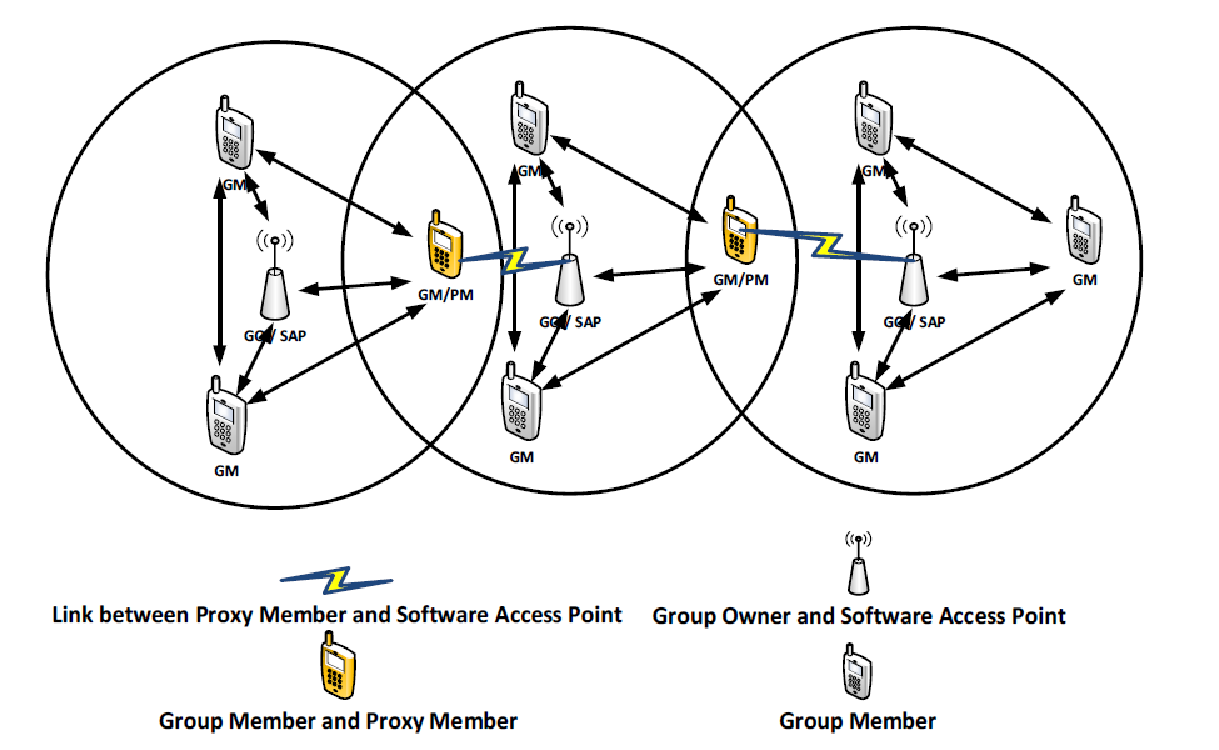
\includegraphics[width=1\textwidth]{images/emc.pdf}}
	\caption{\label{fig:emc} Example of a network topology after running EMC (source: \cite{emc})}
\end{figure}

After the group is created and \gls{PM} selected, the \gls{GO} waits for a period of time before tearing down the group and restarting the EMC protocol. This is done to ensure that the battery drain of the \gls{GO} is minimal and that groups can be established with all the devices for the maximum period of time. Upon restart, the new \gls{GO} is elected and the process is repeated.

In order to overcome the limitations of stock Android already discussed, the authors decided to modify Android's source code. By doing this, multi-group bidirectional unicast communication is allowed. Also, the issue of \gls{IP} addresses assignment is mitigated by giving \glspl{GO} different addresses.

Finally, in order to validate the protocol the authors created a chat application, which runs autonomously without any user interaction, apart from the messages to be sent. Manual override buttons are also present in the application for users to manually control the group creation and teardown.\newline

K. Liu \textit{et al.} propose a new implementation of \gls{MANET}
 using Wi-Fi Direct in stock Android, in \cite{manet}. It is the authors' belief that \glspl{MANET} using this technology can be used in \gls{LTE} offloading systems. This implementation has the following properties:

\begin{itemize}
\item All devices must have the same setup, \textit{i.e.} same functionalities.
\item The devices must be ready to be discovered, connected and to transmit
\item The \gls{MANET} is dynamic so devices must be able to join different groups in the network
\item All devices are able to leave or join the network, making the \gls{MANET} not depend on any device
\end{itemize}

This solution follows a different approach than the previously presented. According to the authors, in order to achieve all of the properties listed above, all devices must become \glspl{GO} when there is no data transmissions, creating a topology similar as the one in Figure \ref{fig:manettop}.

\begin{figure}[ht]
	\noindent\makebox[\textwidth]
    {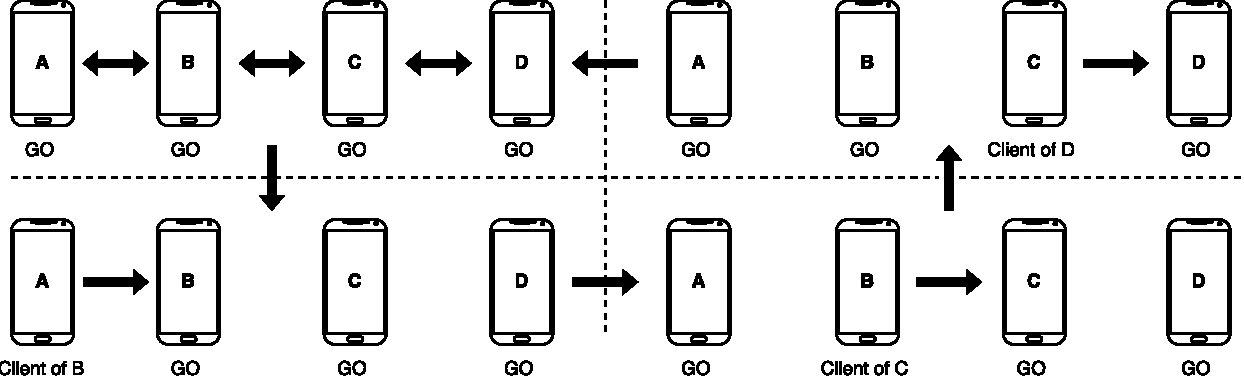
\includegraphics[width=1\textwidth]{images/manettop.pdf}}
	\caption{\label{fig:manettop} Wi-Fi Direct MANET topology (adapted from: \cite{manet})}
\end{figure}

The transmission cycle is as follows: the device with data to transmit must first remove its \gls{GO} status and connect to the destination as \gls{GM}, via the Wi-Fi Direct interface. Once the connection is established, the devices may communicate between them. After the transmission, the device acting as a \gls{GM} disconnects from the group and becomes a \gls{GO} again. This cycle is repeated whenever there is data to transmit.

This \gls{MANET} topology is implemented in stock Android devices, as previously mentioned, and presents a distinct solution from the other works, since the devices in the network are constantly changing roles and groups inside the \gls{MANET}. One disadvantage of this solution is that the status change of the devices are triggered by human interaction with the application, making the network somewhat dependent on human interaction.

\subsection{Multi-Hop Routing}
\label{subsection:mhoprouting}

In the previous section some methods proposed by different authors were presented, in order to create a multi-group networks using Wi-Fi Direct. In this section the focus will be the routing algorithms implemented over some of these methods.

In \cite{routeMultiGroup}, C. Casetti \textit{et al.} propose a content-centric routing algorithm on top of the network topology proposed. Meaning each node knows what is the next hop to which it has to send the request for a specific content - see \cite{contentcentric} for a detailed explanation on content-centric networks.

The authors introduce two data structures responsible for storing the information for content routing: \glspl{CRT}, providing the next hops to reach a certain content. These tables function similarly to standard \gls{IP} routing tables. They store the MD5 hash of the \gls{IP} address of the next hop.

There are three possible scenarios for filling the \gls{CRT}:
\begin{itemize}
\item The simplest one where the content item is available within the group of the content requester, where the next hops of the all \glspl{GM} is the \gls{IP} address of the content provider.

\item The second scenario is when the content is available in a different group, reachable through the group's relay node. This means the \gls{GO} of the second group is connected as a legacy client to the first group and, according to the authors' scheme, all the \glspl{GM} of the first group will have as next hop the group's relay node, except for the \gls{GO} acting as a client. The next hop for the relay client is the \gls{IP} address of the \gls{GO} of the second group. Finally, the next hop of the latter is the \gls{IP} address of the P2P interface of the content provider.

\item The other scenario is when the content is available in a second group, reachable through the \gls{GO} of the first group, which acts as a legacy client in the second group. Following the authors' scheme the next hop for all members of the first group is the \gls{IP} address of the P2P interface of the \gls{GO} acting as a legacy client. The \gls{GO} of the first group will have as next hop the \gls{IP} address of the second group's relay node. The relay client will then follow the steps from the first scenario.
\end{itemize}

The other data structure are the \glspl{PIT}, where the information about the destination of the content item is stored, they are the next hops from the reverse path of the content requests. When forwarding a content request, the nodes store the \gls{IP} address of the node interface from where the request was received. With this mechanism, a "memory" of the content request path is created and utilized to then forward the content item to its requester. Upon receiving the content, the intermediate nodes forward the packet and remove the corresponding entry from the \gls{PIT}. When multiple \gls{PIT} entries requested the same content, the sending node replicates the packet and sends it to all the requesting devices, deleting all the corresponding entries. A content received by an intermediate node without any correspondent entry in the \gls{PIT} is discarded.

The content registration, advertisement and request is done in two phases: the initial phase when a client advertises that new content is available, sending a message to the \gls{GO}, which returns an \gls{ACK} as confirmation. The \gls{GO} will then advertise within the group the availability of the new content, by sending a broadcast message to all \glspl{GM} and waits confirmation from the relay node. This broadcast message is discarded at the \gls{IP} layer by the legacy clients that are \glspl{GO} of other groups. Thus, in order to create a multi-group advertisement, the relay client will send an advertisement to these clients and waits for the \gls{ACK}.

\begin{figure}[ht]
	\noindent\makebox[\textwidth]
	    {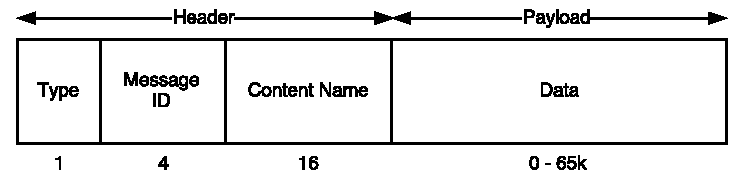
\includegraphics[width=1\textwidth]{images/packet.pdf}}
	\caption{\label{fig:packet} Application-layer message for content registration, advertisement, request and delivery. (adapted from: \cite{routeMultiGroup})}
\end{figure}

The message format can be seen in Figure \ref{fig:packet}, where "Type" refers to the purpose of the message, \textit{i.e.}, Content registration, Content advertisement, Content data, Content request, Relay election or notification of \gls{GO} role in another group and corresponding \glspl{ACK}. "Message identifier" is used to identify what message is an \gls{ACK} referring to. Content name is the MD5 hash of the content name. "Data" is the payload and can carry control or content data.\newline

K. Liu \textit{et. al} also provide a multi-hop routing implementation in \cite{manet}. The authors create a routing table composed by two sub-tables, one containing all peers that are directly discovered by the node and the other composed by peers that are accessible via other peers, \textit{i.e.}, multi-hop peers.

The first sub-table is created with a simple broadcast of the peer discovery signal and it will receive the responses from the devices in the vicinity, since in the authors' topology all devices are \glspl{GO} if no data is being transmitted. The response messages should contain the \gls{MAC} address of the destination devices, the gateway to reach the devices, in this case the node itself, since all nodes are neighbors and the number of hops to reach them, in this case zero.

After the first sub-table is complete all the nodes in the network have knowledge on who are their immediate peers. The nodes will then exchange routing table information between themselves to get a knowledge of all the multi-hop peers that may exist in the network. The second sub-table is filled proactively when nodes receive routing messages. The message-processing scheme is as follows: the device receives a message and checks its destination. If the destination \gls{MAC} is not the device's \gls{MAC} the device will look at its routing table and verify if an entry exists with that destination and where should the message be sent to, incrementing the number of hops, otherwise there is no route to the destination. If the destination \gls{MAC} is the device's \gls{MAC}, it will check the message type and infer if it is a routing message. If so, the device's routing table will be updated with the \gls{MAC} address of the source of the message, the \gls{MAC} address from where the node received the message, \textit{i.e.}, the gateway, and the number of hops necessary to reach the source.

\begin{figure}[ht]
	\noindent\makebox[\textwidth]
    {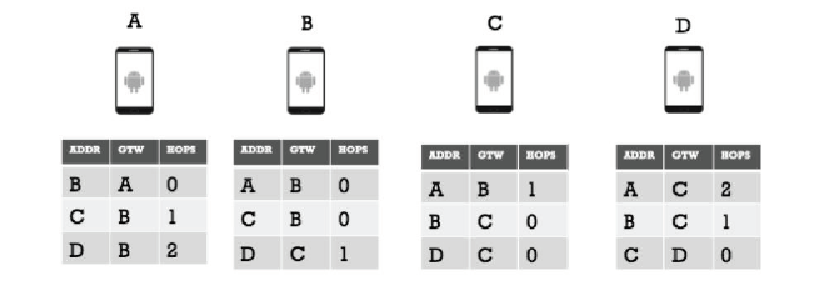
\includegraphics[width=1\textwidth]{images/routeTables.pdf}}
	\caption{\label{fig:routeTables} Wi-Fi P2P MANET routing table. (source: \cite{manet})}
\end{figure}

In Figure \ref{fig:routeTables} it is possible to see a complete table for four different nodes. Each node is now capable of sending a packet to its destination, without having to use a broadcast mechanism.

Two different routing mechanisms have been introduced in this section. Each mechanism is supported by a specific network scheme. This is the main problem of routing in Wi-Fi Direct, since the routing algorithm is developed at the application layer thus being always dependent on implementation, making most of the algorithms not compatible among themselves. This problem also brings some limitations in the number of users that will integrate a specific network with a specific routing scheme.












